\documentclass[compress, blue, 13pt,hyperref={pdfpagemode=FullScreen}]{beamer}
\usepackage{emerald}
\usepackage[T1]{fontenc}
\usetheme{Goettingen}
\usepackage[utf8]{vietnam}
\usepackage[english]{babel}
\usepackage{amsmath}
\usepackage{tikz}
\usepackage{amsfonts}
\usepackage{multimedia}
\usepackage{xcolor}
\usepackage{color}
\usepackage{graphicx}
\usepackage{amssymb}
\usepackage{graphicx}
\usepackage[absolute,overlay]{textpos}
\usepackage{calligra}
\usepackage{mathpazo}
\usepackage{eso-pic}
\usetikzlibrary{shadows}
\usepackage{animate}
\usetikzlibrary{mindmap,trees}
\usepackage{adjustbox}
\usepackage{amssymb}
\usepackage{multicol}
\setlength{\columnseprule}{0.5pt}
\def\columnseprulecolor{\color{blue!80}}
\setbeamerfont{footnote}{size=\tiny}
%\renewcommand{\footnoterule}{}
\beamertemplatenavigationsymbolsempty
\newcommand\AtPagemyUpperLeft[1]{\AtPageLowerLeft{%
\put(\LenToUnit{0.882\paperwidth},\LenToUnit{0.88\paperheight}){#1}}}
\AddToShipoutPictureFG{
  \AtPagemyUpperLeft{{
\includegraphics[width=1cm,keepaspectratio]{images/LogoBK.png}}}
}%



\setbeamertemplate{footline}[frame number]
\author[]{
\includegraphics[width=2cm]{images/LogoBK.png}\\ { }}
\title[]{Thiết kế \& Hiện thực \\ Điều khiển Robot người }
\logo{
\includegraphics[scale=.4]{images/LogoBK.png}}
\institute[Khoa Khoa Học \& Kỹ Thuật Máy Tính, Đại Học Bách Khoa - Tp.HCM]{Trường Đại Học Bách Khoa Tp.HCM \\ Khoa Khoa Học \& Kỹ Thuật Máy Tính  \\ 
\vspace{0.5cm}
\begin{tabular}{ll|llcc}
GVHD&TS.Phạm Hoàng Anh& & Sinh viên thực hiện: &&  \\
GVPB&TS.Lê Trọng Nhân&1. &Nguyễn Hương & $\displaystyle{-}$ & 1411646\\
&&2.&Bùi Thanh Tùng&$\displaystyle{-}$&1414517 
\end{tabular} 
}
\setbeamertemplate{footline}[text line]{%
  \parbox{\linewidth}{\vspace*{-15pt}  \hfill\insertframenumber}}
\setbeamertemplate{navigation symbols}{}
\newcounter{sauvegardeenumi}
\newcommand{\asuivre}{\setcounter{sauvegardeenumi}{\theenumi}}
\newcommand{\suite}{\setcounter{enumi}{\thesauvegardeenumi}}
%\setbeamercovered{transparent} 
%\setbeamertemplate{navigation symbols}{} 
%\institute{} 
\date{} 
%\subject{} 
\begin{document}

%\section*{Outline}
%\begin{frame}
%\tableofcontents
%\end{frame}


\begin{frame}
\titlepage
\end{frame}
\small{
\begin{frame}{Outline}
\tableofcontents
\end{frame}
}
%\section{Giới thiệu}
\section{Mục tiêu đề tài}
\begin{frame}{Mục tiêu đề tài}
\begin{itemize}
\item Thực hiện các tư thế chuyển động giống người.
\begin{itemize}
\item Quay trái
\item Quay phải
\item ...
\end{itemize}
\item Hiện thực các phương pháp giao tiếp và điều khiển robot người thông qua wifi, BLE, tay cầm.
\item Tìm hiểu thiết kế cơ khí của Robot.
\item Tìm hiểu máy tính nhúng
\begin{itemize}
\item Công cụ hỗ trợ 
\item Tạo service
\end{itemize}
\item Lập trình Android cơ bản
\begin{itemize}
\item Thiết kế giao diện
\item Socket 
\item API Google
\end{itemize}
\end{itemize}
\end{frame}
%\subsection{Giới hạn đề tài}
%\begin{frame}{Giới thiệu}{Giới hạn đề tài}
%\begin{itemize}
%\item Hiện thực một số chuyển động cơ bản.
%\item Việc điều khiển Robot không thông qua Internet. 
%\end{itemize}
%\end{frame}

\section{Phương pháp tiếp cận}
\subsection{Phần cứng}
%{
% \setbeamertemplate{footline}{}
\begin{frame}{Phương pháp tiếp cận}{Phần cứng}
\begin{figure}[hbtp]
\centering
\begin{multicols}{2}
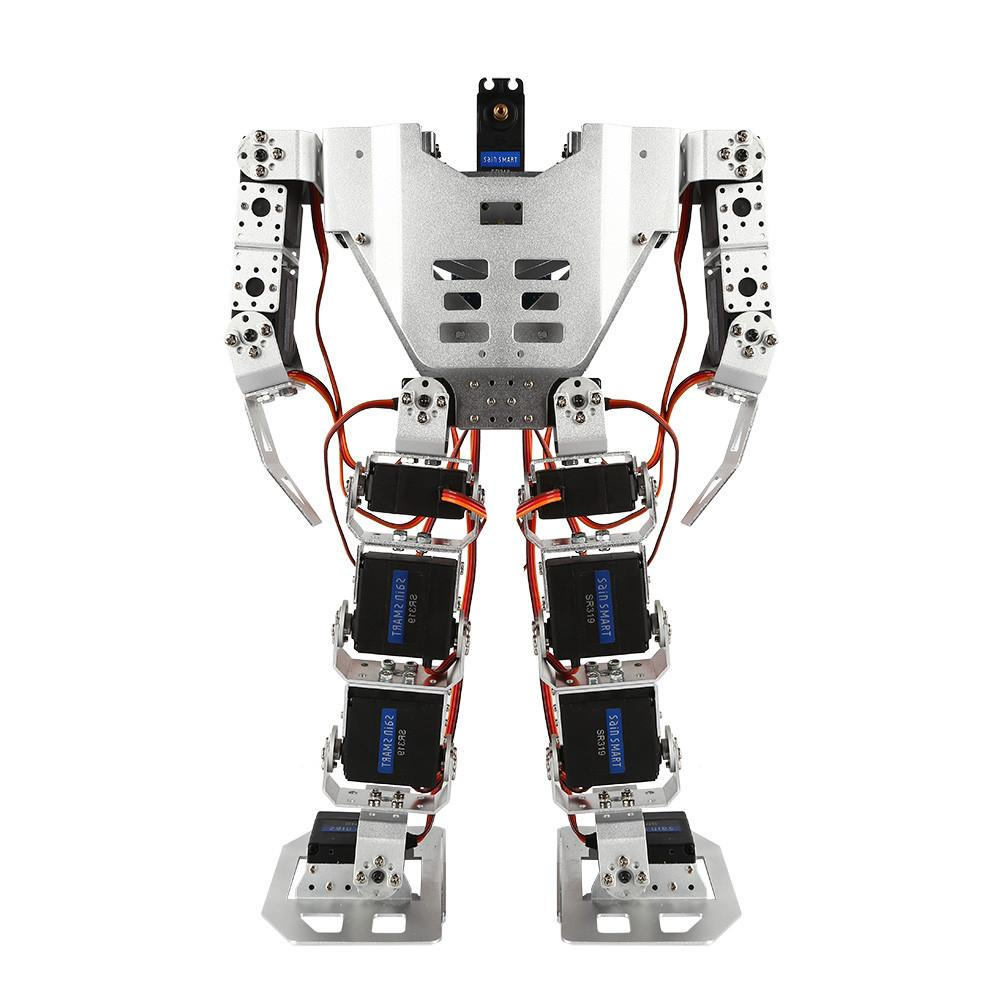
\includegraphics[scale=0.15]{images/01_150_2_1024x1024.jpg}
\columnbreak

\begin{itemize}
\item Kích thước: 320x120x505mm
\item Khối lượng: 1.65KG  3.6lb  
\vspace{0.4cm}
\item Điện áp: 5-7.4V
\item Hệ thống vận hành:  Thay đổi xung PWM truyền vào
\item Nhiệt độ hoạt động: $-10^{o}C\thicksim50^{o}C$
\item Tốc độ: $sec/60^{o}$  %: có thể lên tới :$16Kg.cm/0.14sec/60^{o}@7.4V$
\end{itemize}
\end{multicols}
\caption{Robot-16DOF}
\end{figure}
\footnotetext[1]{https://www.sainsmart.com/products/sainsmart-17-dof-biped-humanoid-kit}
\end{frame}
%}
\begin{frame}{Phương pháp tiếp cận}{Phần cứng}
\begin{figure}[hbtp]
\centering
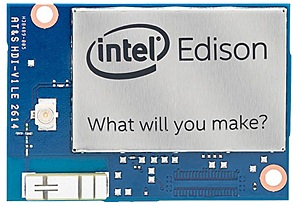
\includegraphics[height = 2cm]{images/MakerBoards-Edison.jpg}
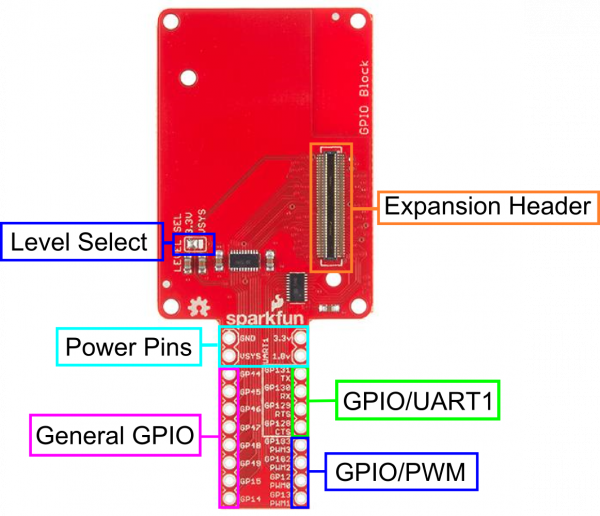
\includegraphics[height = 2.4cm]{images/GPIOBlockAnnotated.png}
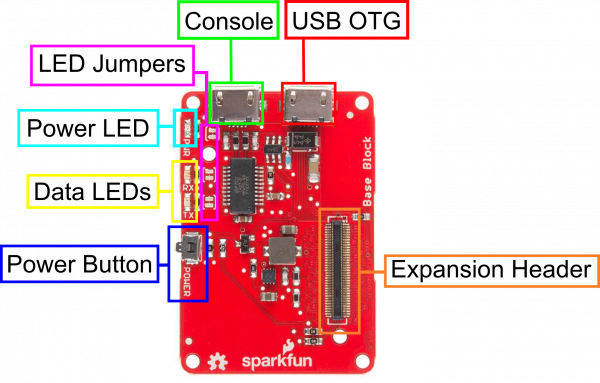
\includegraphics[height = 2.4cm]{images/BaseAnnotated.png}
\caption{Bộ board Intel Edison}
\end{figure}
\end{frame}
\subsection{Mô hình chuyển động của robot}
\begin{frame}{Phương pháp tiếp cận}{Mô hình chuyển động của robot}
\begin{figure}[hbtp]
\centering
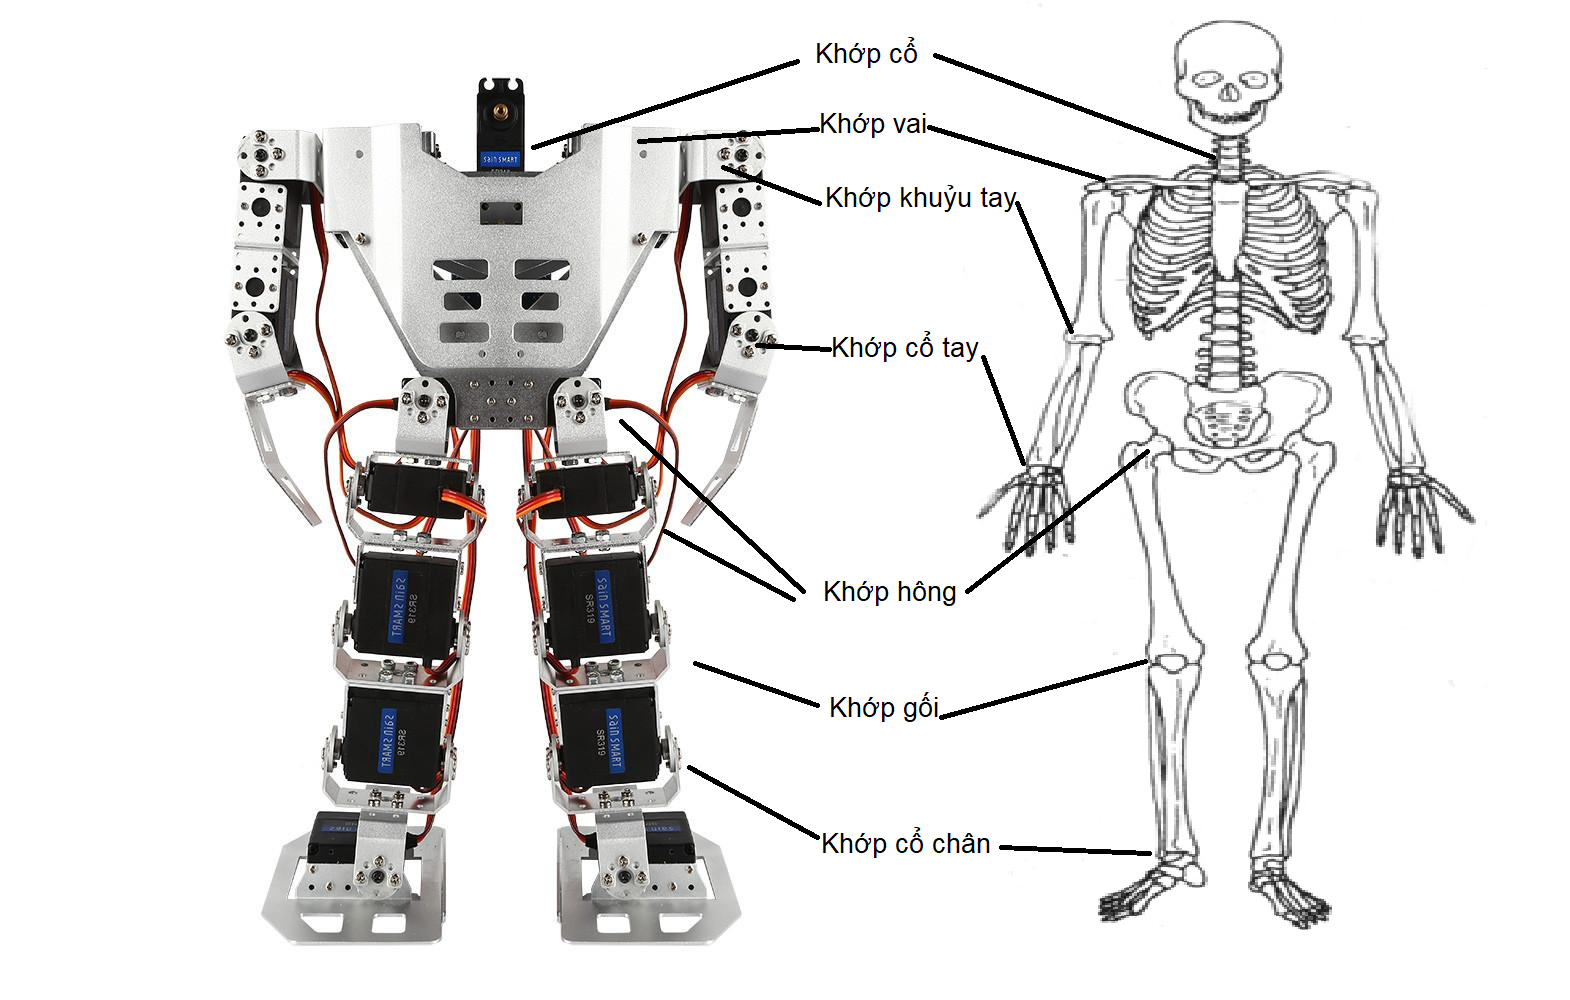
\includegraphics[scale=0.22]{images/ThietkeRobot.png}
\caption{Cấu tạo các khớp của robot}
\end{figure}
\end{frame}
\subsection{Công cụ hỗ trợ phát triển}
\begin{frame}{Phương pháp tiếp cận}{Công cụ hỗ trợ phát triển}
\begin{figure}[hbtp]
\centering
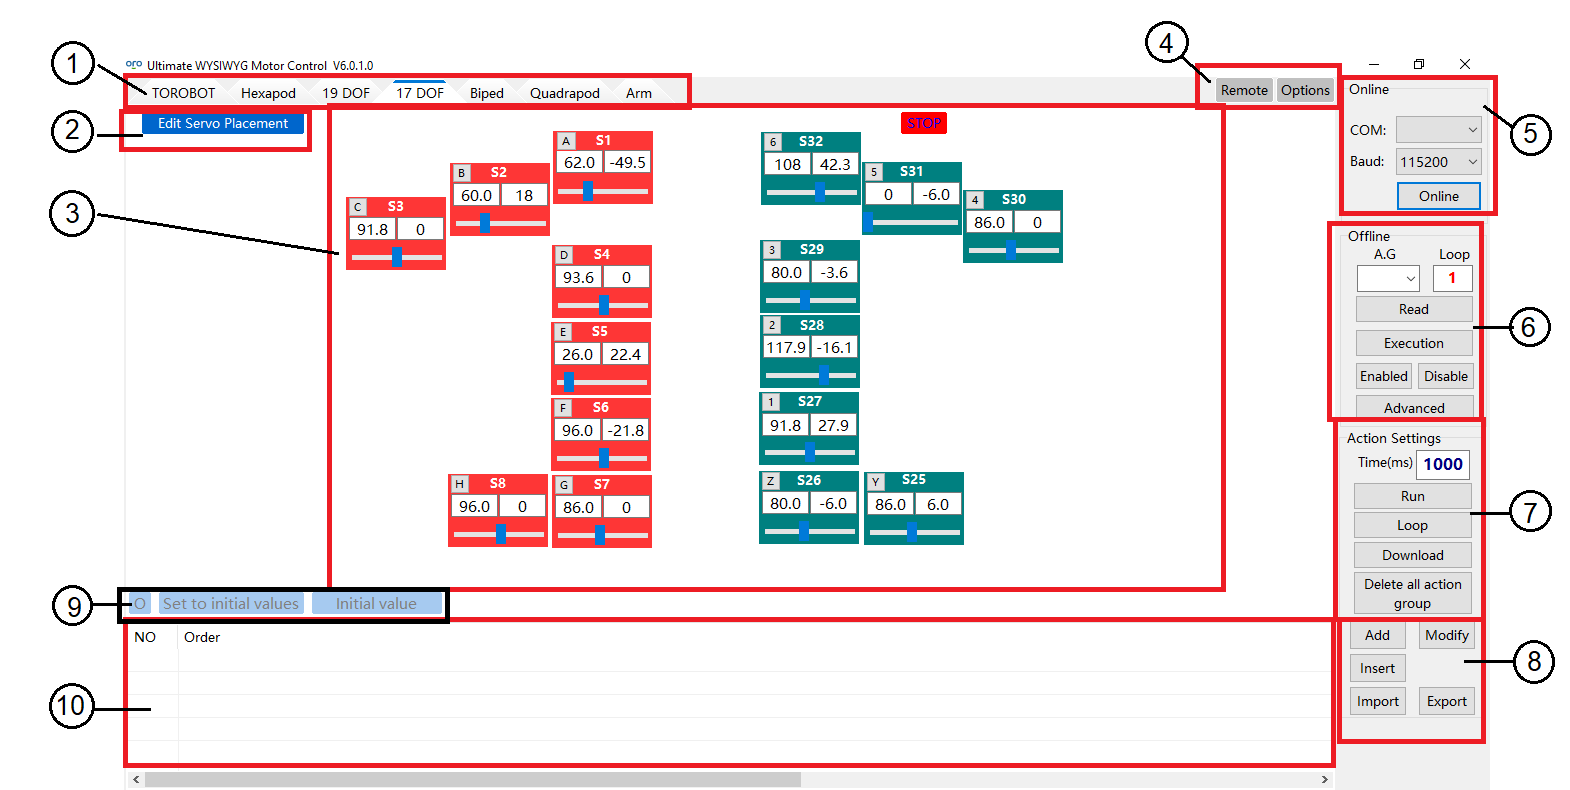
\includegraphics[scale=0.22]{images/Torobot.png}
\caption{Giao diện phần mềm Torobot}
\end{figure}

\end{frame}
\section{Thiết kế \& Hiện thực}
\subsection{Mô hình hệ thống}
\begin{frame}{Thiết kế \& Hiện thực}{Mô hình hệ thống}
Phương thức điều khiển:
\begin{itemize}
\item Wifi
\begin{itemize}
\item Botton(Web)
\item Voice App
\end{itemize}
\item BLE
\item Tay cầm
\end{itemize}
\end{frame}
\begin{frame}{Thiết kế \& Hiện thực}{Mô hình hệ thống}
\begin{figure}[hbtp]
\centering
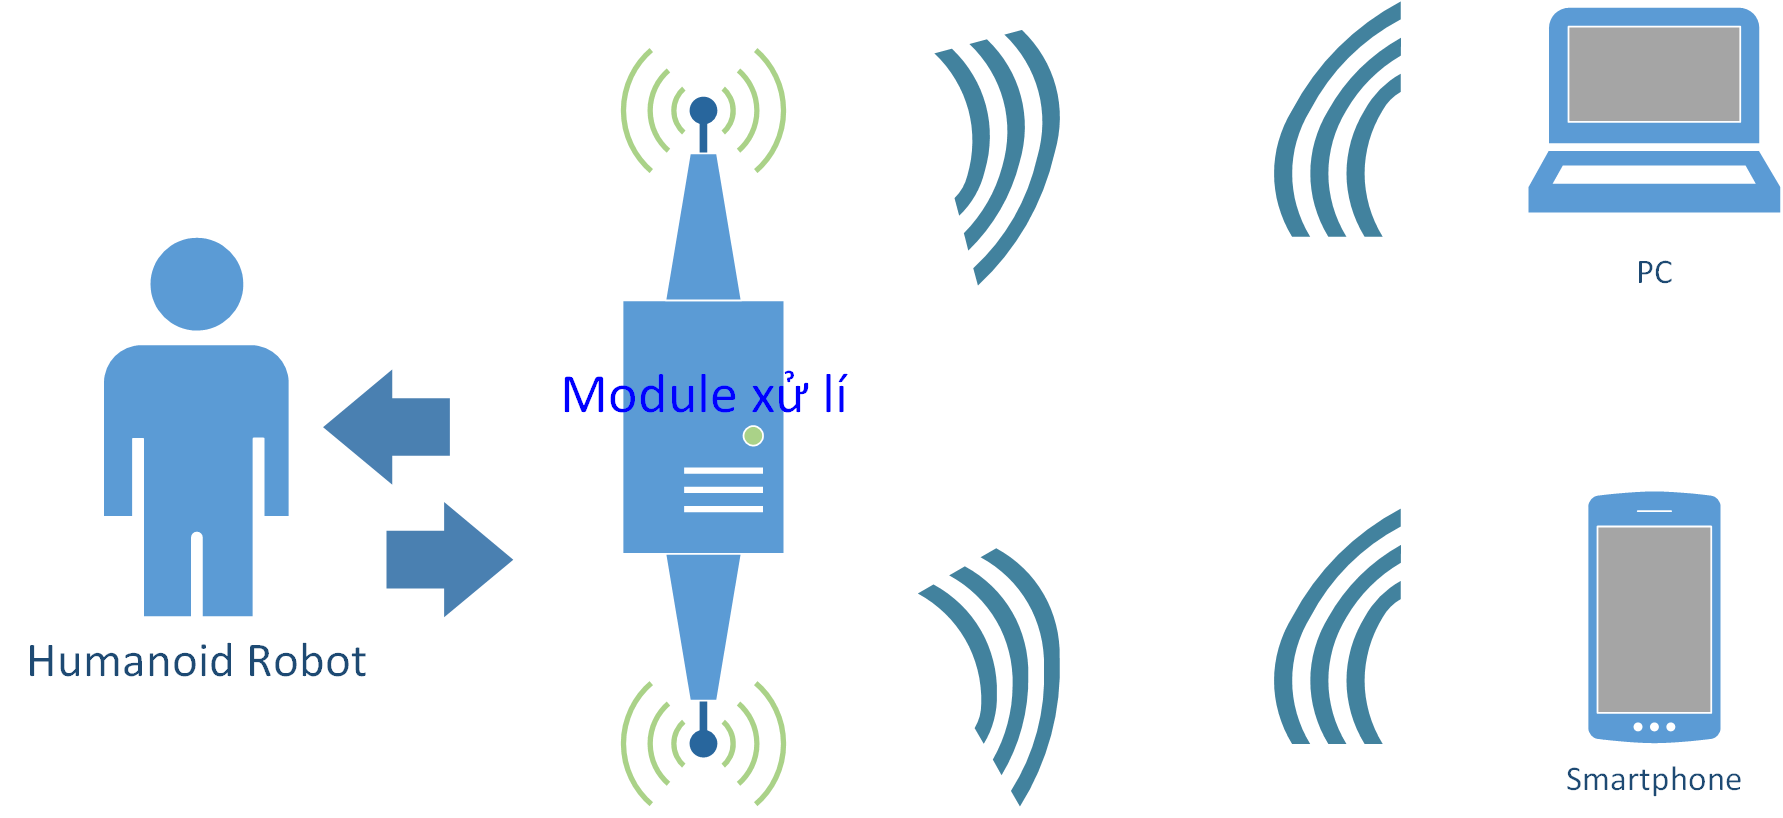
\includegraphics[scale=0.5]{images/protocol.png}
\caption{Giao thức kết nối}
\end{figure}
\end{frame}
\subsection{Module xử lí chính}
\begin{frame}{Thiết kế \& Hiện thực}{Module xử lí chính}
\begin{figure}[hbtp]
\centering
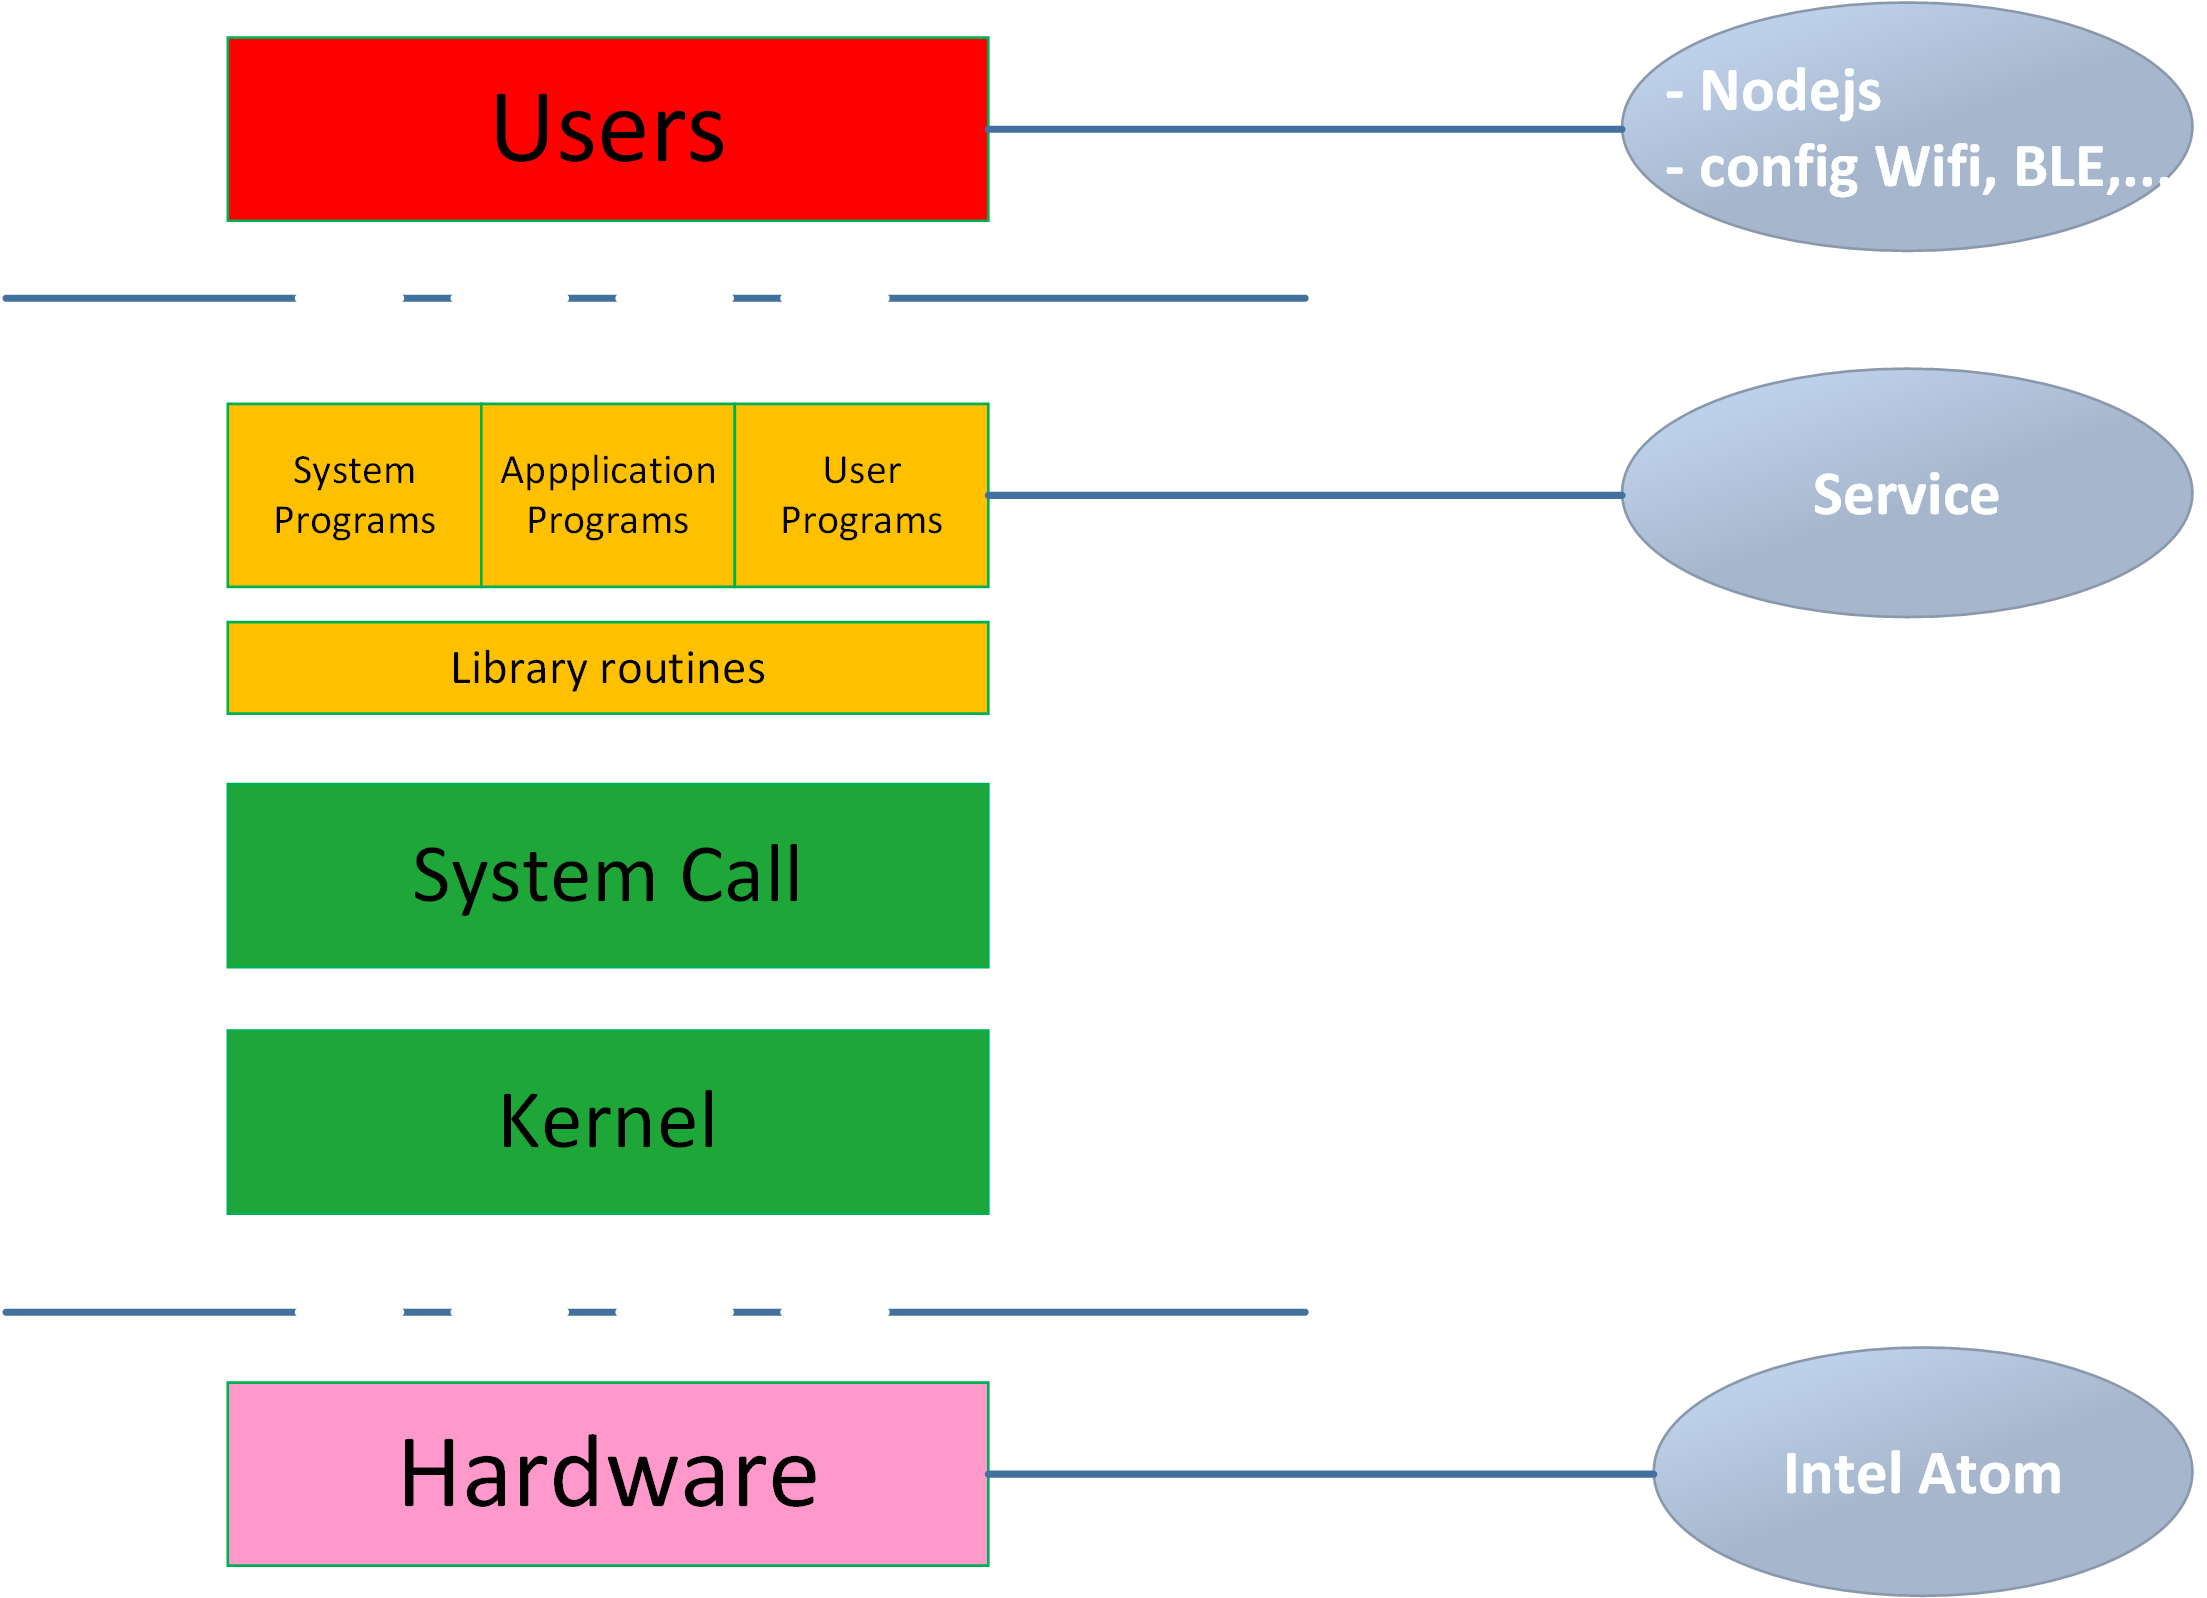
\includegraphics[scale=0.4]{images/architecture_os.png}
\caption{Cấu trúc tổng quát}
\end{figure}
\end{frame}
\begin{frame}{Thiết kế \& Hiện thực}{Module xử lí chính}
\begin{figure}[H]
\begin{adjustbox}{max totalsize={1\textwidth}{0.7\textheight},center}
\begin{tikzpicture}[mindmap, grow cyclic,align=flush center, every node/.style=concept, concept color=orange!80, text=black!90, scale= 0.9,
    level 1/.append style={level distance=4cm,sibling angle=72},
    level 2/.append style={level distance=3cm,sibling angle=55},
    level 3/.append style={level distance=2cm,sibling angle=38},
    level 4/.append style={level distance=3cm,sibling angle=30}]

\node[scale = 0.7]{Ứng dụng}
    child [concept color=blue!75] { node {Package}
    	child[sibling angle=95]{ node{mraa}}
        child[] { node {Nodejs}
			child[]{node{bleno}} 
			child[]{node{http}
				%child[level distance=2cm,sibling angle=-90,concept color=blue!60]{ node{ESP-8266}}			
			}       
			child[]{node{express}
			}
			child[]{node{morgan}
			}
			child[]{node{path}
			}
			child[]{node{mraa}
			}
        }     
    }
    child [concept color=yellow!70] { node {Kết nối}
        child { node {Wifi}}
        child { node {BLE}}
    }
    child [concept color=green!75] { node {Cấu trúc}
        child [sibling angle=110] { node {server}
			child[concept color=green!55]{node {}}
			child[concept color=green!55]{node{}}
			child[concept color=green!55]{node{}} 
        }
        child[] { node {web}
			child[concept color=green!55]{node{css}}
			child[concept color=green!55]{node{html}}
			child[concept color=green!55]{node{JS}}         
        }
    }
    child [concept color=red!70] { node {Ngôn ngữ}
        child []{ node {JavaScript}   
        }
        child [] { node {html}
        }
        child []{ node {css}}
    };

\end{tikzpicture}
\end{adjustbox}
\caption{Mô hình ứng dụng trên Intel Edison}
\end{figure}
\end{frame}
\subsection{Module điều khiển}
\begin{frame}{Thiết kế \& Hiện thực}{Module điều khiển}{1. Web}
\begin{figure}[hbtp]
\centering
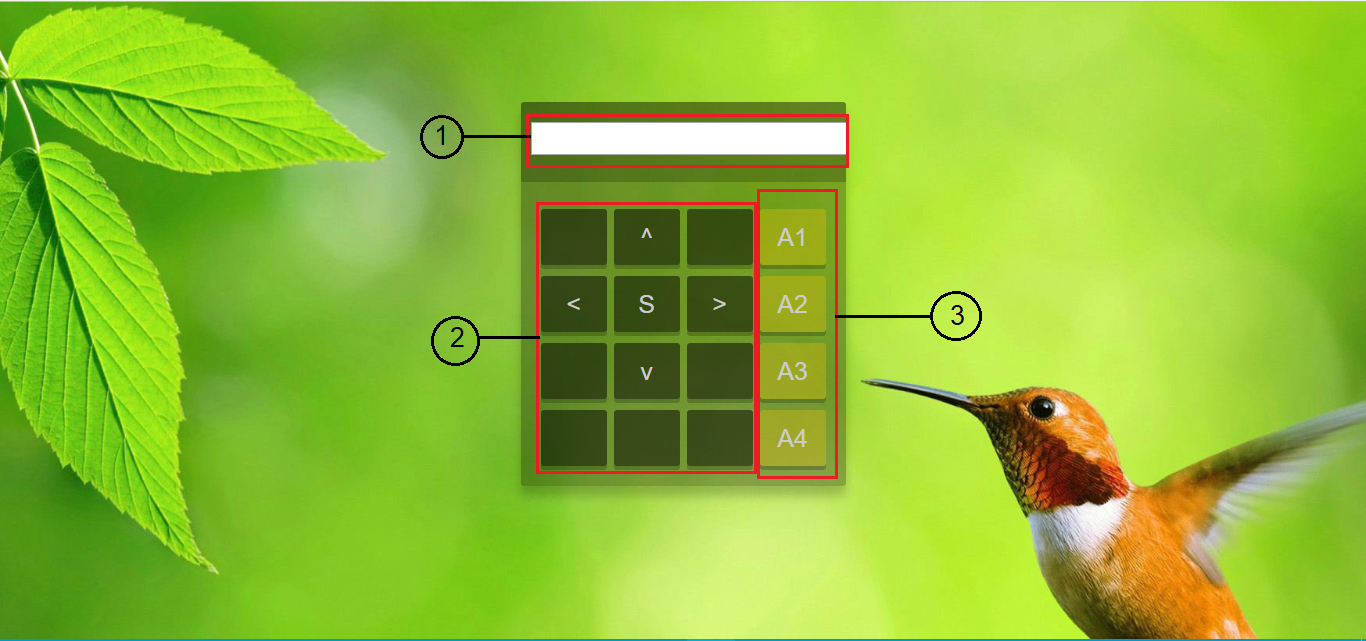
\includegraphics[scale=0.25]{images/web_layout.PNG}
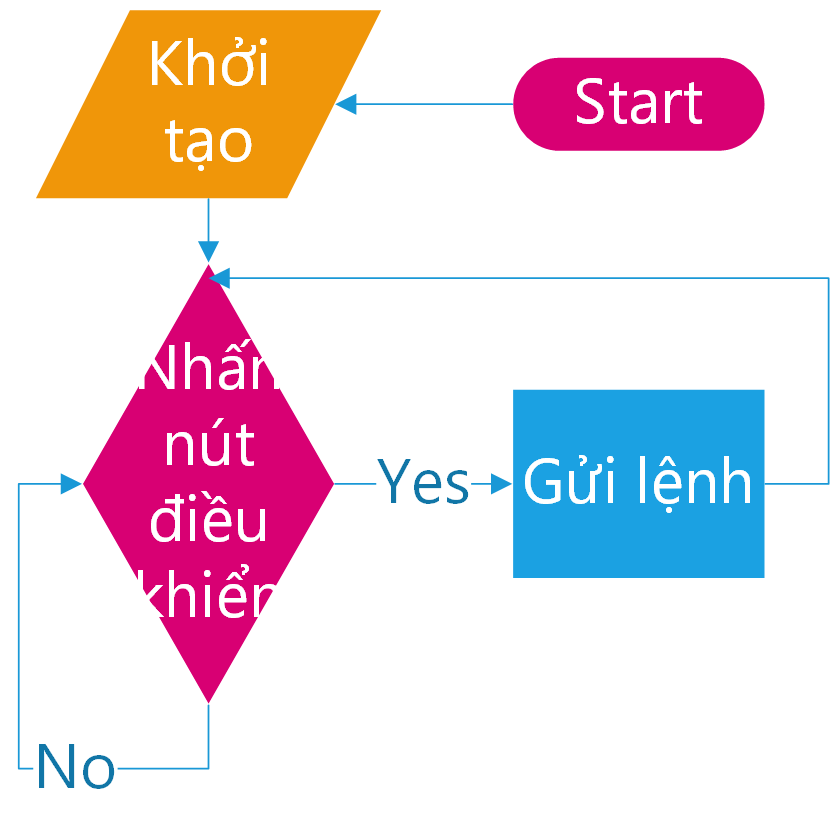
\includegraphics[scale=0.6]{images/flowchart_web.png}
\caption{Giao diện, flowchart  Web}
\end{figure}
\end{frame}
%\begin{frame}{Thiết kế \& Hiện thực}{Module điều khiển}{1. Web}
%\begin{figure}[hbtp]
%\centering
%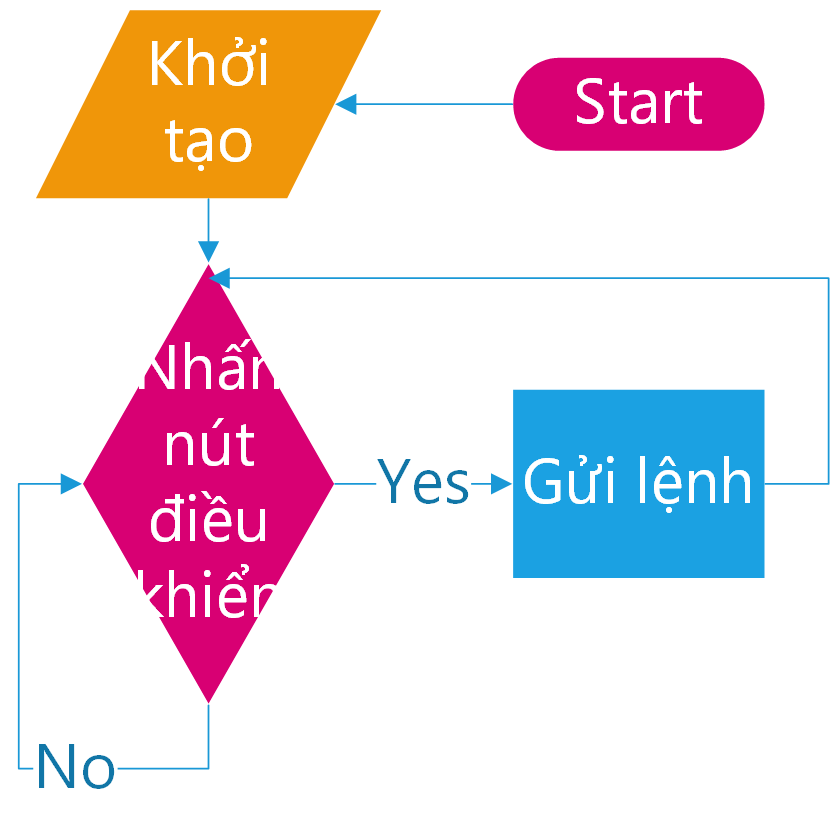
\includegraphics[scale=0.6]{images/flowchart_web.png}
%\caption{Flowchart hoạt động}
%\end{figure}
%\end{frame}
\begin{frame}{Thiết kế \& Hiện thực}{Module điều khiển}{2. Android App}
\begin{figure}[hbtp]
\centering
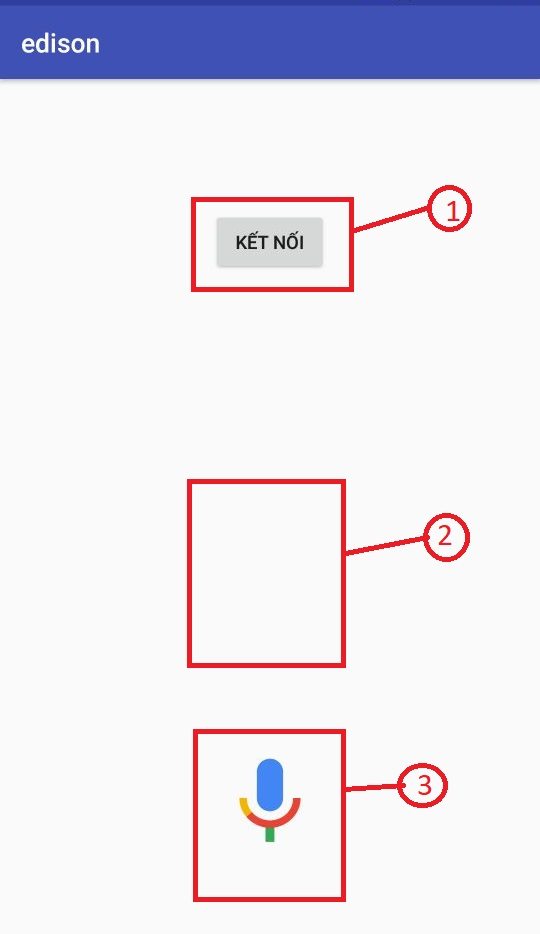
\includegraphics[scale=0.22]{images/1528618723907.JPEG}
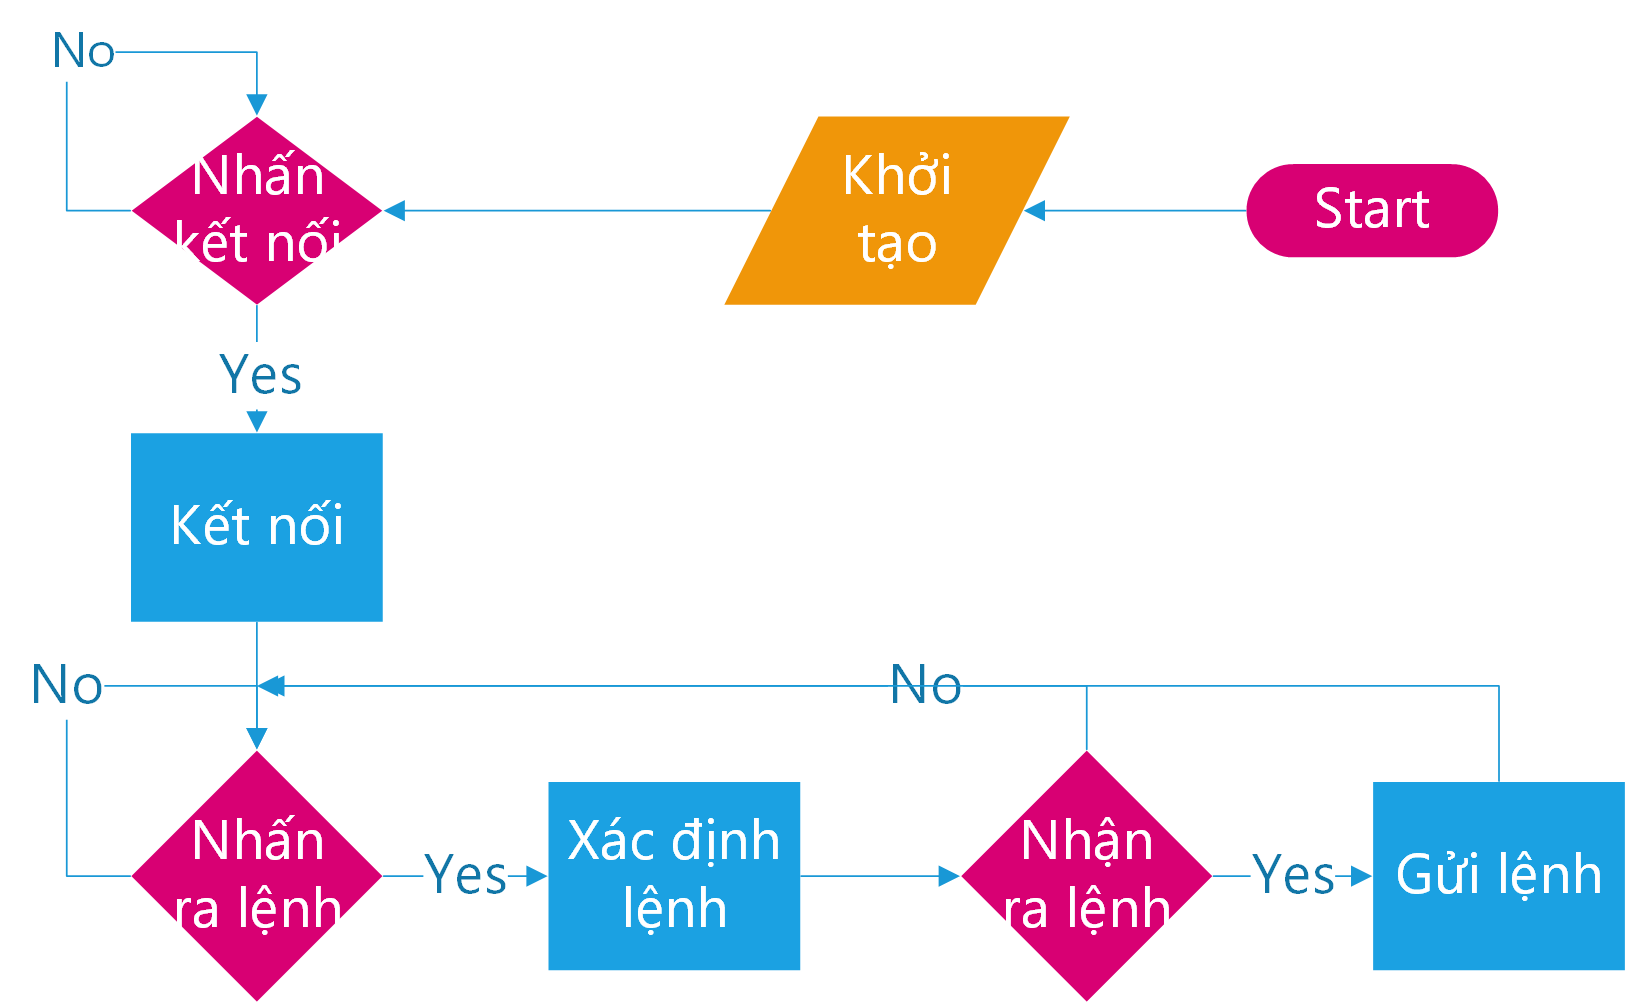
\includegraphics[scale=0.43]{images/flowchart_app.png}
\caption{Giao diện, flowchart App giọng nói}
\end{figure}
\end{frame}
%\begin{frame}{Thiết kế \& Hiện thực}{Module điều khiển}{2. Android App}
%\begin{figure}[hbtp]
%\centering
%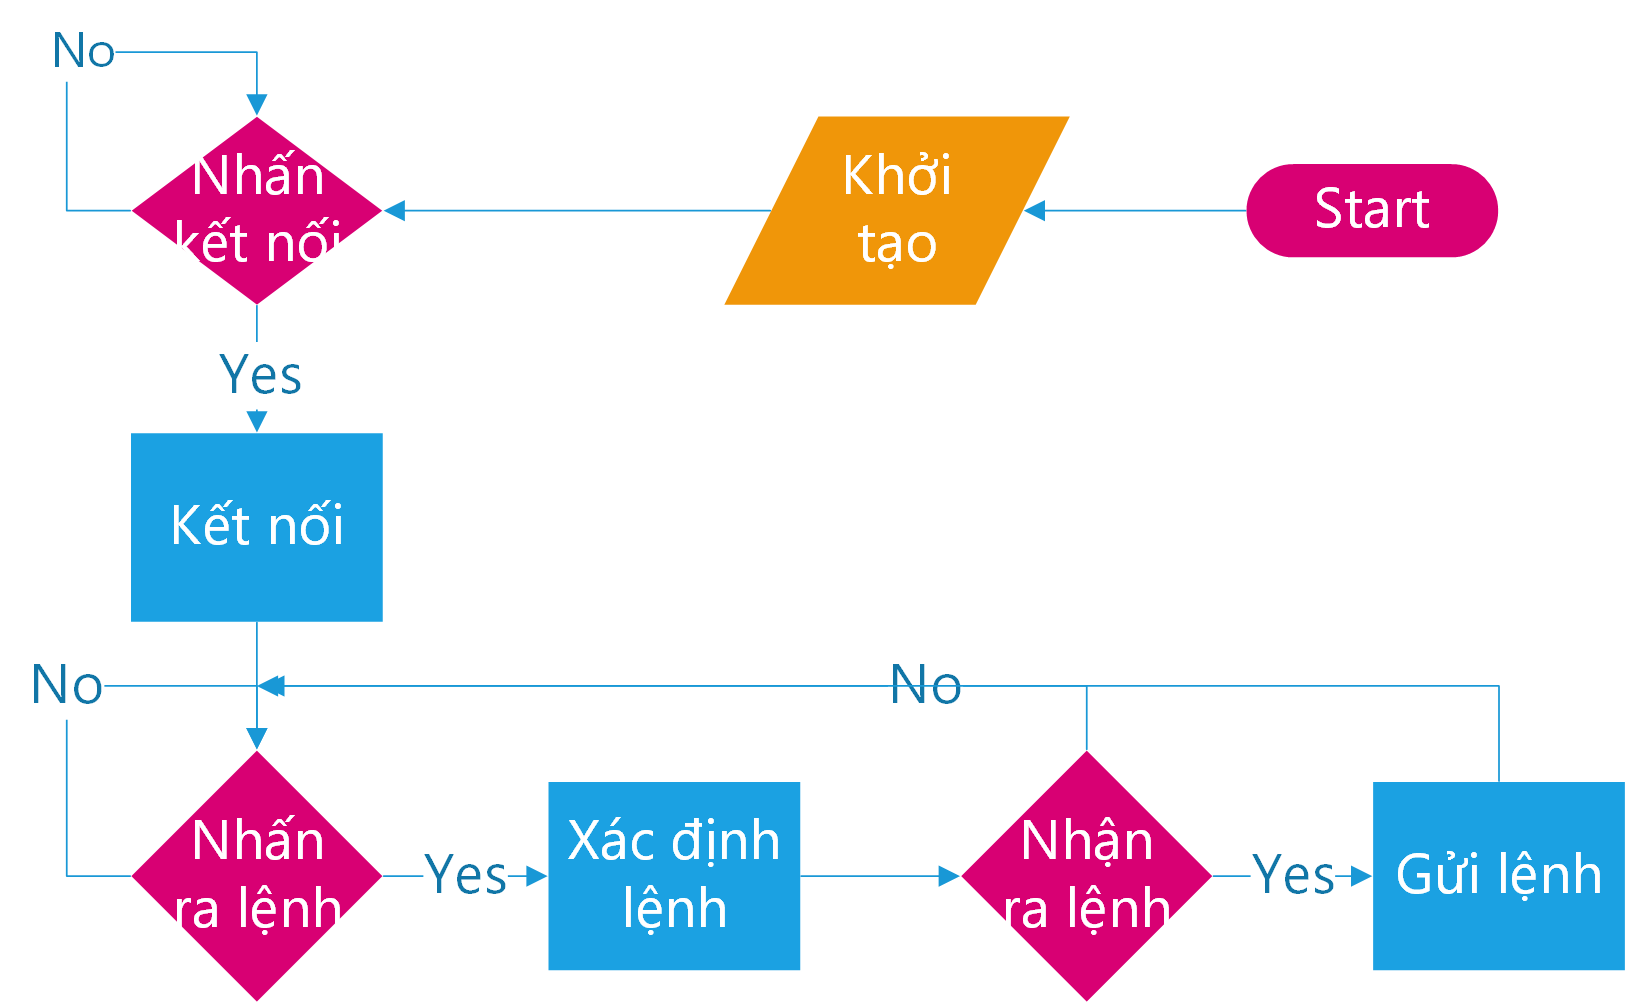
\includegraphics[scale=0.45]{images/flowchart_app.png}
%\caption{Flowchart hoạt động}
%\end{figure}
%\end{frame}
\begin{frame}{Thiết kế \& Hiện thực}{Module điều khiển}{2. Android App}
\begin{figure}[hbtp]
\centering

\includegraphics[scale=0.4]{images/nRF.png} 
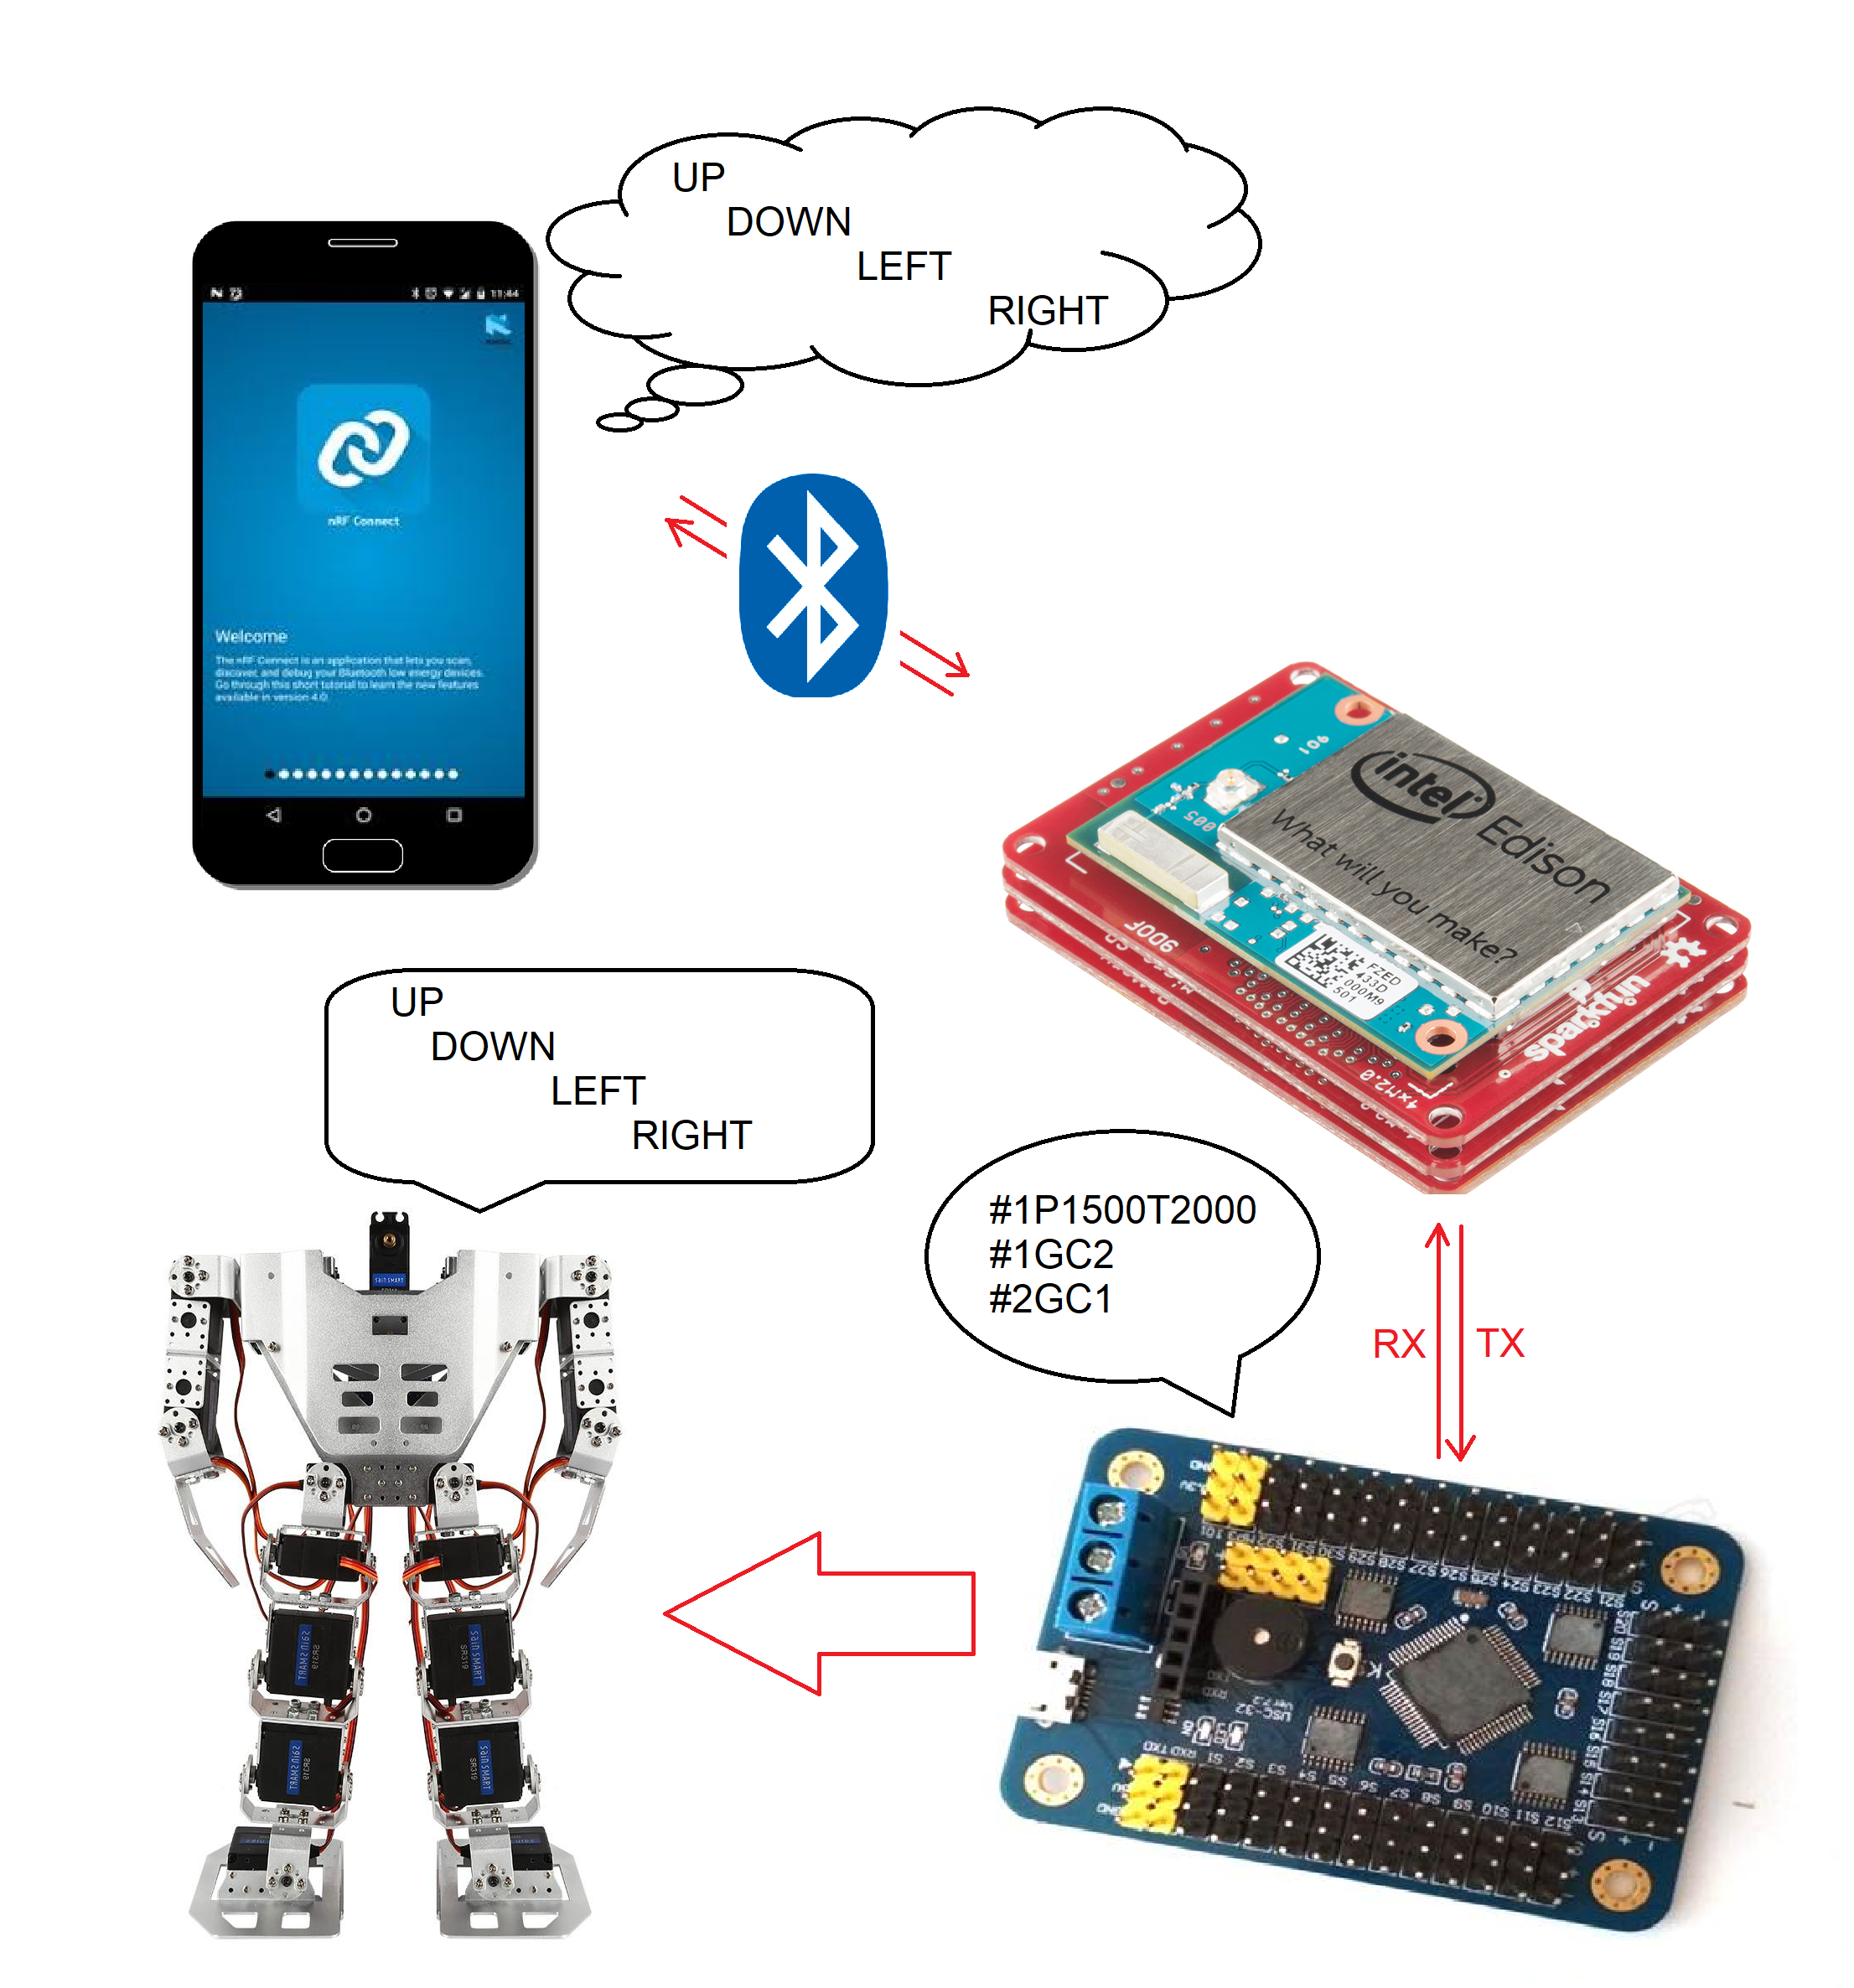
\includegraphics[scale=0.07]{images/BLEApp.png} 
\caption{App điều khiển thông qua BLE}
\end{figure}
\end{frame}
\begin{frame}{Thiết kế \& Hiện thực}{Module điều khiển}{3. Tay cầm}
\begin{figure}[hbtp]
\centering
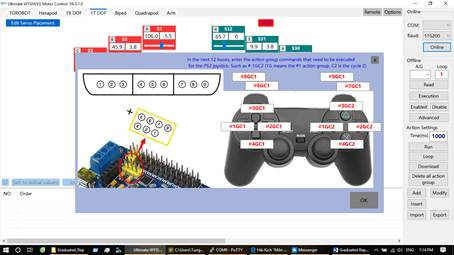
\includegraphics[scale=0.43]{images/image007.jpg}
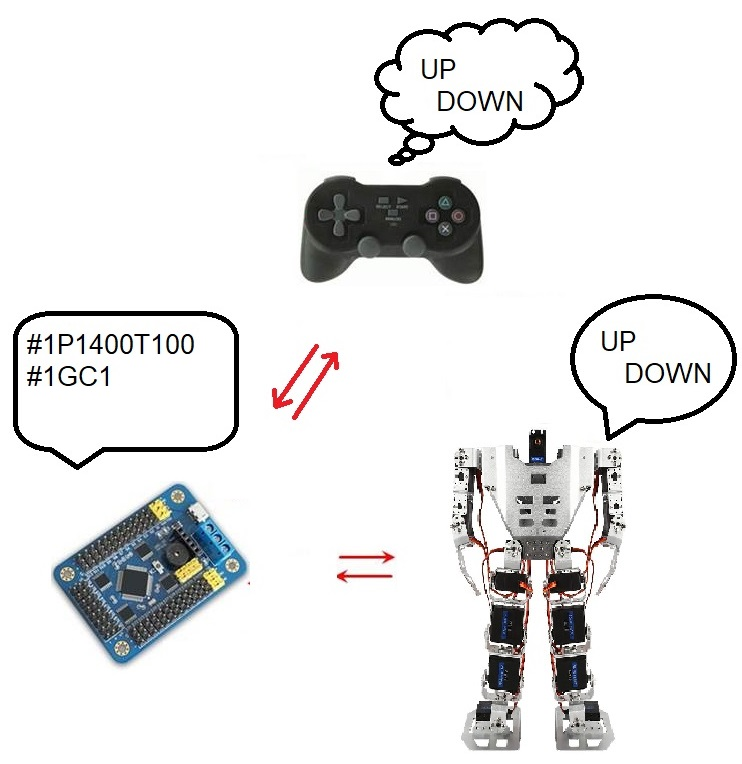
\includegraphics[scale=0.25]{images/PS2GamePad.jpg}
%\caption{}
\end{figure}
\end{frame}
%\subsection{Chuyển động của robot}
%\begin{frame}{Thiết kế \& Hiện thực}{Chuyển động của robot}
%
%\end{frame}
\subsection{Tư thế đã hiện thực}
\begin{frame}{Thiết kế \& Hiện thực}{Tư thế đã hiện thực}
\begin{multicols}{2}
{
\begin{itemize}
\item Đi thẳng
\item Quay trái
\item Quay phải
\item Sang trái
\item Sang phải
\item Đá bóng
\item Mang đồ vật
\end{itemize}
}
\columnbreak

\begin{figure}[hbtp]
\centering
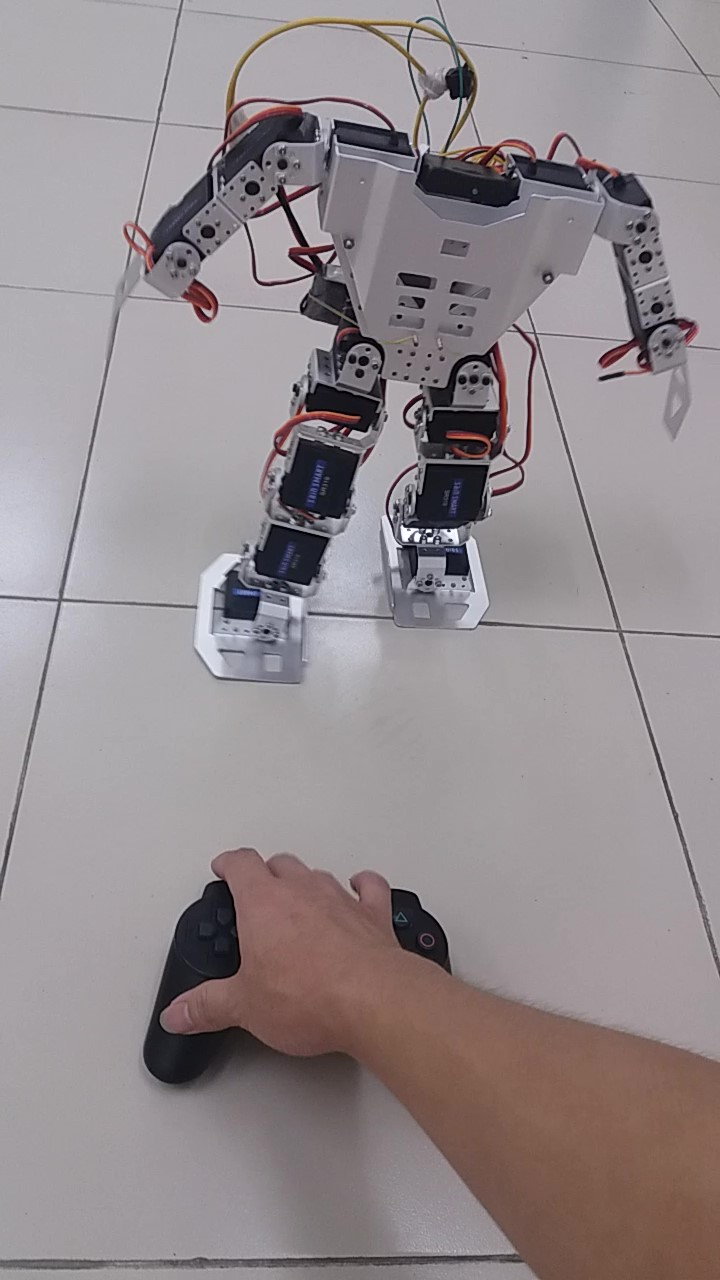
\includegraphics[scale=0.1]{images/Results/RotateLeft.jpg}
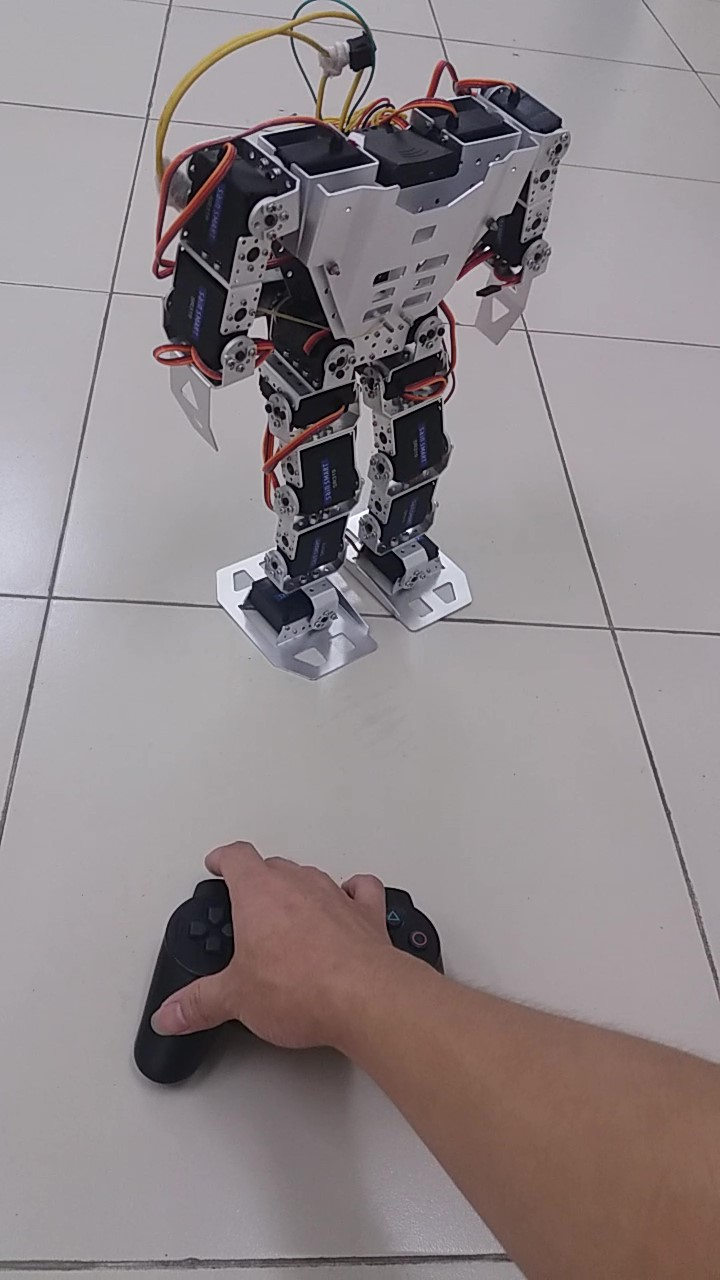
\includegraphics[scale=0.1]{images/Results/RotateLeft2.jpg}
\caption{Robot sang trái}
\end{figure}

\end{multicols}
\end{frame}
\section{Kết luận}
\subsection{Kết quả đạt được}
\begin{frame}{Kết luận}{Kết quả đạt được}
\begin{itemize}
\item Hiểu rõ cấu tạo, nguyên lý thiết kế phần khung cơ thể và cách chuyển động của robot.
\item Sử dụng được Intel Edison và phần mở rộng.
\item Thiết kế App Android.
\item Giao thức kết nối.
\end{itemize}
\end{frame}
\subsection{Khó khăn}
\begin{frame}{Kết luận}{Khó khăn}
\begin{itemize}
\item Lưu ý điện áp của Intel Edison
\item Đụng độ socket.
\item Tạo domain name cho Intel Edison.
\item Tài liệu tham khảo từ Torobot đa số bằng tiếng Trung.
\item Điều chỉnh trọng tâm theo từng tư thế.
\end{itemize}
\end{frame}
\subsection{Hướng phát triển}
\begin{frame}{Kết luận}{Hướng phát triển}
\begin{itemize}
\item Nhúng thêm sensor để robot di chuyển một cách tự động
\begin{itemize}
\item Sensor siêu âm: tránh vật cản
\item Sensor hồng ngoại: di chuyển theo đường cho trước
\item IMU sensor: tự động cân bằng
\end{itemize}
\item Phát triển những tư thế phức tạp hơn:
\begin{itemize}
\item Nhảy cóc, tự đứng dậy khi ngã
\item Lên xuống cầu thang
\item Đấm, đá, thủ thế...
\end{itemize}
\item Chia chế độ hoạt động:
\begin{itemize}
\item Balancing Mode
\item Soccer Mode
\item Fighting Mode
\item Carry Mode
\end{itemize}
\end{itemize}
\end{frame}
\subsection{Tham khảo}
\begin{frame}{Tham khảo}
\begin{thebibliography}{39}
\addcontentsline{toc}{chapter}{Tham Khảo}
%\bibitem{Luque:2003}
%Applying UML and Patterns:
%\textit{An Introduction to Object-Oriented Analysis and Design and
%Iterative Development, $3^{rd}$ Edition - 2004 - Craig Larman}.
%\bibitem{Slides}
%Slides,
%\textit{Bài giảng bộ môn Công Nghệ Phần Mềm (Thầy Lê Lam Sơn - 2017)}.
\bibitem{website1}URL: \url{http://hshop.vn/products/mach-dieu-khien-32-rc-servo}.
\bibitem{website2}URL: \url{https://communities.intel.com/docs/DOC-111103}
\bibitem{website4}URL: \url{http://www.instructables.com/id/Intel-Edison-BLE-Controlled-Lights/}
\bibitem{website5}URL: \url{https://github.com/noble/bleno}
\bibitem{website9}URL: 
\url{https://communities.intel.com/docs/DOC-102152}
\bibitem{website12}URL: \url{https://www.youtube.com/watch?v=i5fpbxNwLyc}
\bibitem{website13}URL: \url{https://www.youtube.com/watch?v=AC9XpWkmU7k}
\bibitem{website14}URL: \url{https://www.youtube.com/watch?v=W6CUzogyjUI}
\end{thebibliography}
\end{frame}
\section*{}
\begin{frame}
\transdissolve
\begin{center}
\begin{Huge}
\color{blue}{Cảm ơn các thầy/cô đã lắng nghe}
\end{Huge}
\end{center}
\end{frame}
\end{document}